\documentclass[12pt]{article}
\usepackage[margin=1in]{geometry}
\usepackage{graphicx}
\usepackage{hyperref}
\usepackage{amsmath}
\usepackage{float}
\usepackage{makecell}
\newcolumntype{C}[1]{>{\centering\arraybackslash}m{#1}}
\usepackage{enumitem}
\usepackage{url}
\usepackage{tikz}
\usetikzlibrary{arrows.meta, positioning}
\usepackage{caption}
\usepackage{booktabs}
\usepackage{longtable}
\usepackage[utf8]{inputenc}
\newcommand{\rupee}{Rs.}
\usepackage{natbib}                 % for author–year citations
\bibliographystyle{elsarticle-harv}    
\providecommand{\DOIprefix}{}
\renewcommand{\DOIprefix}{}
\providecommand{\doi}[1]{#1}
\renewcommand{\doi}[1]{\href{https://doi.org/#1}{https://doi.org/#1}}
\usepackage[linesnumbered,ruled,vlined]{algorithm2e}
\usepackage{amsmath}
\tikzstyle{decision} = [diamond, draw, fill=blue!20, text width=5em, text centered, inner sep=0pt]
\usepackage{authblk}
\usepackage{subcaption}
\usepackage[toc,page]{appendix}
\usetikzlibrary{arrows.meta,positioning,shapes.geometric,shapes.misc,fit,calc}
\usepackage{lipsum} % for dummy text
\DeclareUnicodeCharacter{202F}{\,} % or simply a regular space: {\ }
\tikzset{
	entity/.style={rectangle, draw, rounded corners, minimum height=1cm, minimum width=2.5cm, align=center},
	process/.style={ellipse, draw, minimum height=1cm, minimum width=3cm, align=center, fill=blue!10},
	data/.style={rectangle, draw, minimum height=1cm, minimum width=2.5cm, align=center, fill=yellow!20}
}

\usepackage{tikz}
\usetikzlibrary{shapes.geometric, arrows.meta, positioning}
\usepackage{setspace}
%\setstretch{2}

\title{Privacy-Conscious Federated Reinforcement Learning for Blockchain-Enabled Adaptive Finance in Agri-Food Supply Chains}



\author{Dhanish Jose and Pradeepmon T G}  
\affil{Department of Mechanical Engineering,\\ National Institute of Technology Calicut, India}





\date{}


\begin{document}
	
	\maketitle
	
	\begin{abstract}
	Delayed payments to farmers, opaque auction practices, and limited access to working capital for wholesalers continue to weaken liquidity, trust, and repayment discipline in the Indian cardamom supply chain. This study proposes a Hyperledger Fabric-based supply chain finance framework that integrates produce traceability, auction settlement, packet-level sales, and adaptive financing within a permissioned blockchain architecture. Reinforcement Learning (RL) determines the financier-side base Annual Percentage Rate (APR), while Federated Reinforcement Learning (FL-RL) enables multiple financiers to improve borrower screening collaboratively. Each financier trains on its own repayment and profitability records, and only model updates are aggregated; raw client identities, account-level histories, and complete transaction records remain with the originating institution. The final offered APR combines the RL-selected base APR with a borrower-specific RL risk premium subject to predefined APR limits.
	
	The FL-RL mechanism was evaluated against isolated RL borrower screening across four random seeds, three capital levels, and four default-severity scenarios. Across 48 matched comparisons, FL-RL achieved a higher return in 45 cases, increasing mean return on initial capital from 32.81\% to 41.08\%, producing approximately 8.09M greater cumulative net profit, and reducing the mean loan-count default rate by 4.60 percentage points. In the 1M high-default scenario averaged across seeds, FL-RL increased return from 106.56\% to 139.53\% while reducing the default rate from 9.12\% to 1.84\%.
	
	The findings indicate that combining portfolio-level RL-based APR adaptation with federated borrower-side RL screening can improve capital performance and repayment-risk control without pooling raw client records. Hyperledger Caliper benchmarking further confirms the feasibility of executing the main smart-contract workloads in the proposed permissioned blockchain network. The study contributes a privacy-conscious collaborative finance framework for high-value agricultural auctions while identifying the need for multi-seed validation and stronger formal privacy mechanisms in future deployment.
	\end{abstract}
	
	
	
	
	
Keywords: Cardamom supply chain; Supply chain finance; Hyperledger Fabric; Blockchain auction; Adaptive APR; Federated Reinforcement Learning; Privacy-conscious borrower screening; Smart contracts; Agri-food traceability
	
	
	
	\section{Introduction}
	
	Small cardamom (Elettaria cardamomum (L.) Maton), celebrated as the "Queen of Spices," forms the economic backbone of thousands of smallholder farmers in the Western Ghats of Kerala, India (\cite{murugan_governance_2024}). Despite their high export potential and market value, cardamom cultivation is highly expensive and labour-intensive, with the average cultivation cost exceeding \rupee~5.9 lakh per hectare (\cite{murugan_governance_2024}). 
	Fertilizers, pesticides, and labour expenses constitute a significant share of cardamom cultivation costs, and the costs are incurred well before any revenue is realised from the crop. Unlike other agricultural products, dried cardamom is a premium product, with recent Spices Board auction listings showing average prices above \rupee{} 3,000 per kg and maximum prices above \rupee{} 4,000 per kg (\cite{spicesboard_daily_price_2026}). In Kerala, most sales of dried cardamom take place through Spices Board-regulated auction centres, and the total value of auction transactions is substantial, which underscores the significance of timely payments and transparent auctions. However, Spices Board auction material and field studies note that delayed farmer payments remain a persistent concern beyond the mandated settlement period (\cite{spicesboard_cardamom_auction,murugan_governance_2024}). This liquidity gap forces farmers operating on thin cash flows to rely on informal financiers. These financiers "discount" the auction bills---providing immediate cash at heavily reduced values---and thereby exploit the structural delay in formal payment cycles. As a result, farmers incur significant financial losses while attempting to bridge the working-capital gap created by delayed auction settlements.
	
	Another menace faced by cultivators is the rampant manipulation of the bidding process within auction centers. The traders frequently engage in repeated bidding on the same lot, a practice that artificially drives down the final settlement price. This often results in artificially depressed prices in favour of the wholesalers. Furthermore, it has the potential to create an unwanted exuberance, which eventually results in a price crash, negatively impacting all stakeholders participating in the supply chain (\cite{reddy_status_2016}).
	
	A related challenge is the farmer's limited practical bargaining power after bids are placed. When the offer is unsatisfactory, the farmer may still have weak ability to reject or renegotiate the outcome. This vulnerability can be exploited by traders who coordinate to suppress prices, disadvantaging smallholder growers. Such coordinated behaviour further entrenches the imbalance within the market and amplifies financial disadvantages faced by farmers (\cite{acharya_agricultural_2004,reddy_status_2016}).
	
	The problem is not limited to farmers; it adversely affects the wholesalers who are denied much-needed working capital owing to unreliable credit histories, lack of collateral, and high risk associated with it. These factors deter the financial institution from advancing loans to the wholesalers (\cite{caniato_supply_2019}). The lack of transparency and the inability of the financier to recover the loan advanced rob them of the business opportunity while negatively impacting the wholesalers who are denied liquidity to settle the transactions of the farmers. This fragmented financial ecosystem magnifies the trust deficit across the value chain, besides amplifying payment defaults and delays (\cite{gelsomino_supply_2016}).
	
	
	Cardamom is a high-value commodity crop, with daily auction transactions in major auction centres reaching substantial monetary value; it is therefore highly vulnerable to the aforementioned operational and integrity issues (\cite{spicesboard_daily_price_2026,spicesboard2023annual,dgcis2023export,murugan_governance_2024}). Although the integration of blockchain into traditional electronic supply and finance systems entails significant upfront and operational costs, it is justified by the high market value and export potential of the commodity.
	
	Existing government interventions and institutional credit schemes do not effectively address the multiple challenges posed by the lack of real-time credit scoring, opaque credit history, and centralized administration.
	The opaque nature of traditional auction systems makes it difficult to trace payments or penalize delayed settlements (\cite{gelsomino_supply_2016}). Therefore, a transparent, data-driven, and adaptive financing mechanism that can continuously assess financial behaviour, rewarding reliability and discouraging deliberate default, is indispensable for the cardamom supply chain.
	
	To address these limitations, the present study proposes a blockchain-based framework coupling electronic auction with RL-driven supply chain finance. The system is demonstrated through a cardamom supply-chain case study and uses Hyperledger Fabric to record authorised events from produce submission and bidding to settlement, finance, sale, repayment, and default. RL is applied at two complementary levels: a portfolio-level agent adapts the financier's base APR, and a borrower-level agent assigns a risk premium from repayment and realised-profit signals. FL extends the borrower-side agent across financiers so that locally learned Q-table updates can be aggregated without centralising complete client records.
	
	Federated Learning (FL) extends this adaptive mechanism across participating financiers. Each institution learns from its own client repayment and profitability records, while collaboration occurs through aggregated model updates rather than through the transfer of raw client identities, account-level loan histories, or commercially sensitive transaction records. The purpose is therefore not unrestricted sharing of client details, but privacy-conscious collaborative learning in which identifiable records remain under the control of the originating financier.
	
The study aims to develop and evaluate an adaptive, privacy-conscious, blockchain-enabled supply chain finance framework for high-value agricultural auctions. The proposed system integrates Hyperledger Fabric-based traceability, smart-contract-driven auction and settlement processes, wallet-based payments, RL-based APR adaptation, and FL-RL borrower screening. Each financier retains its raw client records locally and computes Q-table updates from repayment behaviour, overdue exposure, default occurrence, and realised profitability. Only the model-level values required for aggregation are collaboratively combined. This design seeks to improve risk assessment across financiers without placing directly identifiable client profiles or complete transaction histories in a shared training dataset.

\subsection{Aim and Objectives}

The central aim is to determine whether permissioned blockchain infrastructure and federated adaptive learning can enable financiers to collaborate on borrower-risk assessment while preserving institutional control over sensitive client information. The specific objectives are: (1) to design a Hyperledger Fabric architecture that links produce traceability, auction execution, settlement, finance disbursement, packet sales, and repayment within an authenticated and auditable workflow; (2) to develop an RL-based portfolio module that adapts the financier-side base APR to capital utilisation, repayment outcomes, and realised profitability; (3) to develop a local RL borrower-screening mechanism that transforms repayment and profit behaviour into borrower-specific risk premiums; (4) to implement federated RL screening so that financiers aggregate locally learned Q-table parameters without pooling raw client identities, account-level repayment histories, or full transaction records; (5) to compare FL-RL with matched isolated RL screening across different capital and default-severity conditions, thereby measuring whether collaborative learning improves return and default control; and (6) to evaluate the operational feasibility of the permissioned blockchain through Hyperledger Caliper throughput, latency, and transaction-success benchmarks.

In this study, ``privacy-preserving'' denotes data minimisation, local retention of raw records, permissioned participation, and model-update sharing rather than raw-data exchange. The current prototype does not claim formal differential-privacy or secure-multiparty-computation guarantees; resistance to model-inversion, membership-inference, and malicious-participant attacks remains an important deployment and future-research requirement.
	
	
	
	
	
	
\section{Related Work}

This section summarises the literature needed to position the proposed framework: supply-chain finance and blockchain auctions, adaptive finance using RL and FL, and permissioned blockchain deployment for auditable agricultural workflows.

\subsection{Supply-Chain Finance and Blockchain Auctions}

Supply-chain finance helps address the liquidity shortages faced by intermediaries such as traders and wholesalers, but lending is often constrained by unverifiable credit histories, weak collateral, fragmented information, and perceived repayment risk \citep{stiglitz_credit_1981,rajan_covenants_1995,caniato_supply_2019}. Information sharing between financiers and borrowers strongly shapes SCF performance; limited transparency reduces lending activity and prolongs settlement cycles \citep{moretto_can_2021}. These limitations are acute in agricultural auction settings, where delayed settlement, bid manipulation, and weak traceability can affect both farmer payments and wholesaler liquidity.

Electronic auctions improve bidding and allocation efficiency, but participants still depend on the platform operator for trustworthy record keeping. Prior studies note risks such as bid suppression, collusion, settlement disputes, and limited farmer bargaining power in agricultural markets \citep{reddy_electronic_2019}. Blockchain-based auction studies address related concerns through tamper-evident records, anonymity, bid privacy, fairness, and public verifiability \citep{ye_anonymous_2023,zhang_blockchain-based_2024,liu_when_2024}. However, these works generally focus on auction fairness and integrity rather than linking auction outcomes to credit assessment, working-capital finance, repayment enforcement, and adaptive credit terms.

Blockchain-SCF studies show that distributed ledgers can improve transparency, coordination, settlement reliability, and financing efficiency in multi-party supply networks \citep{li_three-level_2023,hu_acsarf_2025,modgil_blockchain-enabled_2024}. Yet most blockchain-SCF frameworks remain centred on information sharing or rule-based workflow automation. They rarely convert repayment behaviour, overdue exposure, and realised profitability into adaptive lending terms, leaving a gap between ledger-based traceability and behaviour-sensitive finance policy.

\subsection{Reinforcement Learning and Federated Learning for Adaptive Finance}

Reinforcement Learning (RL) has become increasingly relevant for adaptive financial decision-making. \citet{qu2025rules} applied offline RL to interest-rate adjustment in decentralised lending and showed that learned rate policies can respond more flexibly to market stress than rule-based mechanisms. In supply-chain decision-making, \citet{Guo_2025} demonstrated the value of multi-agent learning for distributed optimisation. These studies support RL for adaptive decisions under uncertainty, but they do not address borrower screening across competing financiers that cannot pool raw client histories.

Federated Learning (FL) directly addresses distributed financial data by allowing participants to update shared models without transmitting complete raw records. Recent credit-risk studies use FL for heterogeneous non-IID financial data, positive-and-unlabelled credit scoring, and rural inclusive-finance assessment across banks, cooperatives, platforms, e-commerce providers, and microfinance institutions \citep{li2024dynamicfl,qiu2025hetfedpu,xie2026fedattncredit}. These studies show the promise of collaborative risk learning, but most treat credit scoring as classification or default prediction rather than linking model updates to finance-offer terms such as APR or borrower-specific risk premiums.

The FL literature also cautions that local data retention alone is not a formal privacy guarantee. Differential privacy, homomorphic encryption, secure aggregation, and verifiable aggregation introduce explicit privacy--utility--computation trade-offs \citep{naresh2026privacycredit,wang2025secureaggregation}. Accordingly, the present study uses the term privacy-conscious: raw client records remain local in a permissioned setting, but the current Q-table averaging does not implement formal differential privacy, homomorphic encryption, or cryptographically secure aggregation.

Taken together, the literature supports RL for adaptive finance decisions and FL for collaborative learning under institutional data separation, while highlighting non-IID data, communication cost, privacy leakage, and aggregation integrity as deployment challenges. The missing link is an auditable agricultural SCF workflow that combines portfolio-level RL APR adaptation, borrower-level FL-RL risk-premium learning, blockchain-linked auction outcomes, and smart-contract-enforced repayment.

\subsection{Hyperledger Fabric in Supply Chain Finance}

Hyperledger Fabric is widely used in supply-chain prototypes because its permissioned architecture, membership service, role-based access control, and chaincode model support cross-organisational workflows with auditable but access-controlled records \citep{ma2019,khan2022,shih2022}. Implementations in tea traceability, pharmaceutical distribution, and multi-chain logistics demonstrate its suitability for provenance tracking, auditing, and inter-organisational coordination \citep{chen_hyperledger_2023,sudha_trackchain_2024,chou_implementing_2023}. For auction-linked finance, these features are important because bid records, finance requests, credit evaluation, repayment status, and settlement histories are commercially sensitive and should not be exposed on a public ledger. Fabric therefore provides an appropriate deployment substrate for the proposed cardamom auction and adaptive finance workflow, while transaction throughput and contention behaviour still require empirical benchmarking.

\section{Research Gaps in Adaptive Blockchain-Enabled Supply Chain Finance}

Despite advances in blockchain-enabled supply chain finance (SCF) and auction systems, significant research gaps remain. First, most studies treat traceability, auctions, and financing as isolated modules, failing to link auction outcomes directly with post-auction liquidity requirements. Second, existing blockchain-SCF frameworks typically rely on static or rule-based financing terms that cannot dynamically respond to volatile agricultural markets, capital constraints, or changing borrower repayment behaviours. Third, each financier observes only a partial client history, yet direct pooling of borrower identities, repayment records, defaults, and profitability data across competitors creates confidentiality and governance concerns. Finally, RL and FL are rarely operationalised together as an auditable finance policy within a permissioned auction-and-settlement workflow or evaluated through matched federated and isolated-learning comparisons.
	
	To address these gaps, this study proposes an adaptive, permissioned blockchain-based supply chain finance framework with the following key contributions:
	
	\begin{enumerate}[leftmargin=*]
		\item \textbf{Integrated blockchain architecture:} A Hyperledger Fabric framework that unifies quality testing, auction execution, lot settlement, traceability, and supply chain finance into a single permissioned ledger.
		\item \textbf{Smart-contract automation:} Automated workflows that execute bid reviews, lot settlement, consumer packet sales, and loan disbursements without discretionary delays, ensuring transparent and auditable transaction histories.
		\item \textbf{Adaptive two-level RL mechanism:} A dynamic finance-policy layer combining financier-side RL for base-APR optimisation with borrower-side RL for behaviour-sensitive risk premiums.
		\item \textbf{Federated RL integration:} A privacy-conscious collaborative screening mechanism in which financiers retain raw client records locally and aggregate borrower-screening Q-table updates rather than pooling identifiable histories.
		\item \textbf{Matched federated evaluation:} Scenario-level comparison of FL-RL with isolated RL, together with fixed-rate and no-screening baselines across capital and default-risk conditions.
		\item \textbf{Blockchain benchmarking:} Hyperledger Caliper evaluation of transactional throughput, latency, and success under the proposed permissioned workflow.
	\end{enumerate}
	
	\section{Methodology}
	
	
	
	
	The methodology proposes a unified blockchain architecture integrating traceability, commodity auctioning, and an adaptive RL--FL finance mechanism. Authorised events from produce submission, grading, auction, finance, sale, and repayment are immutably recorded for traceability. Auction rules are enforced automatically to support transparent decisions and timely farmer settlement. Each financier processes its own client repayment and profitability records locally; the federated layer shares and aggregates borrower-screening Q-table updates rather than centralising complete client files. The resulting finance offer reflects both the financier's portfolio position and the borrower's learned risk premium.
	
	
	
	\subsection{Conceptual Framework of the Proposed System}
	
	
	
	
	The conceptual framework is designed to address the structural inefficiencies in the cardamom supply chain by coupling traceability, automated payments, and an adaptive credit mechanism. The architecture is organised into three analytically distinct layers---the 
	Traceability Layer, the Auction Layer, and the Smart Finance Layer---each resolving a specific class of operational or financial bottlenecks. Together, these layers form a closed adaptive loop in which operational data and financial outcomes continuously reinforce one another, enabling real-time policy evolution and trustworthy execution of transactions. Fig.~\ref{fig:ledger-architecture} presents the blockchain-enabled system architecture.
	
	The Traceability Layer establishes the informational backbone of the system by recording all physical supply-chain events---produce submission, quality testing, grading, and auctioning---in an immutable ledger. This eliminates information imbalance, thereby ensuring that downstream financial decisions are taken on trusted observations rather than unverifiable reports. 
	
	The Auction Layer facilitates transparent bidding operations that prevents manipulation and rebidding of lots by recording all auction transactions immutably. It enforces rule-driven auction behaviour through smart contracts and gives autonomy to farmers to accept or reject the bids. Additionally, it provides credible inputs for the downstream finance layer for credit issuance.
	
	The Smart Finance Layer facilitates automated credit issuance, disbursement, and repayment. Smart contract-driven rules guide the credit issuance, replacing human intervention and enforcing revenue-splitting rules for automated repayment. Repayment timing and payoff outcomes are recorded as quantitative behavioural signals, which are used by the adaptive finance-policy layer to update borrower screening and future finance offers. These updated policy outputs directly influence future financial terms, creating a self-regulating ecosystem in which participant performance shapes credit access.
	
	By integrating all the layers into a single unified blockchain architecture, the system ensures information from one layer directly influences the subsequent layers, enabling traceability, transparent auction, and adaptive credit financing. It eliminates discretionary human intervention and strengthens financial discipline and liquidity while ensuring guaranteed automated payments to farmers.
	
	\begin{figure}[!ht]
		\centering
		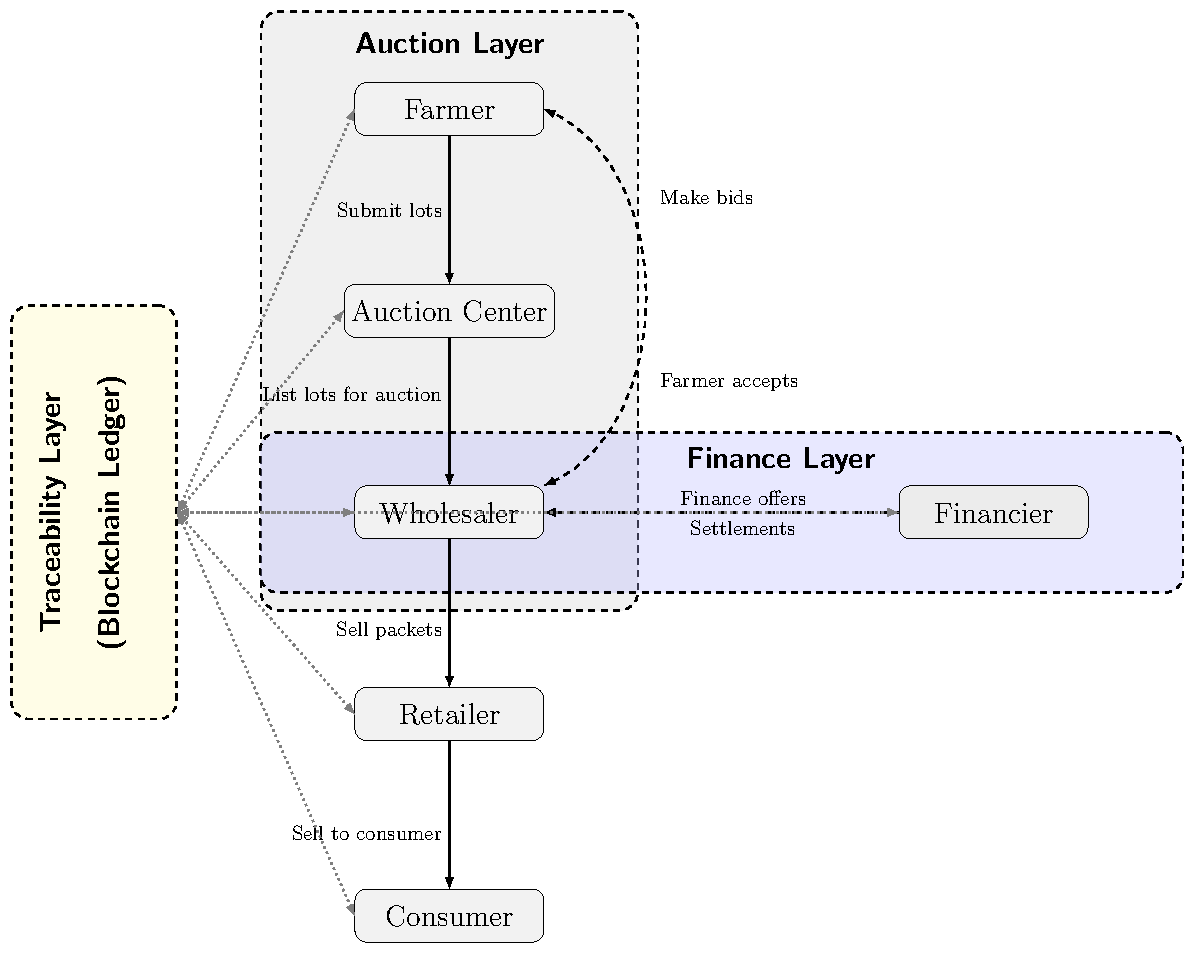
\includegraphics[width=\linewidth]{Figure_1.pdf}
		\caption{Conceptual layered architecture of the proposed system, highlighting the traceability ledger as a foundational layer enabling auction coordination and finance settlement.}
		\label{fig:ledger-architecture}
	\end{figure}
	
	\subsection{Network Architecture}
	
	The proposed system is deployed on a permissioned Hyperledger Fabric consortium network comprising six organisations—each operating an independent peer node and associated Membership Service 
	Provider (MSP). This architecture ensures decentralized validation of transactions while facilitating role-based access control.
	The six organizations are
	\begin{itemize}
		\item Farmers Organization: submits produce lots for auction.
		\item Auction Organization: manages bidding and verifies transactions.
		\item Wholesalers Organization: purchases lots and requests finance.
		\item Retailers Organization: purchases packets from wholesalers and sells packets to consumers.
		\item Financiers Organization: provides liquidity and sets the finance policy
		\item Consumers Organization: purchases individual packets and accesses traceability records.
	\end{itemize}
	
	
	Each organisation operates a dedicated Certificate Authority (CA), which issues cryptographic identities to its users and peer nodes. These identities are validated by the MSP of the organization, allowing the network to authenticate users and enforce access control.
	
	The consortium includes a dedicated orderer node and a Raft-based ordering service. It orders the transactions into blocks and distributes them to peers on the cardamom finance channel for validation. The Raft-based ordering service was configured with a batch timeout of 2 seconds and a maximum batch size of 500 transactions, with a preferred block size of 2 MB and an absolute limit of 10 MB.
	
	
	All the peers are connected through a dedicated channel called cardamom-finance-channel, which provides a shared ledger across all peers and ensures all peers receive the same ordered blocks. Each peer stores its own world state database (CouchDB). Client applications interact with the network using the Fabric Gateway API, which is exposed via a REST interface. Each organisation defines an anchor peer to support gossip-based state dissemination.
	
	
	
	Explicit endorsement policies ensure transaction correctness. Auction transactions require endorsements from WholesalersMSP and FarmersMSP, while finance transactions require endorsements from WholesalersMSP and FinanciersMSP. Retailer bulk-purchase transactions involve WholesalersMSP and RetailersMSP, whereas consumer packet-purchase transactions involve RetailersMSP and ConsumersMSP. This fine-grained endorsement structure enhances trust by ensuring that critical decisions cannot be executed unilaterally.
	
	A single smart contract (cardamom contract) encodes the entire workflow from produce submission, grading, auction, finance, sales, settlement, and repayment-outcome recording. The contract is installed on all peer nodes and invoked using the Fabric Gateway API.
	
	All peer-to-peer and peer-to-orderer transactions are secured using TLS encryption. Every transaction is signed with the submitter’s private key, ensuring non-repudiation and tamper resistance. Fig.~\ref{fig:cardamom-network} illustrates the stakeholders and their peers in the supply chain.
	
	
	\begin{figure}[!ht]
		\centering
		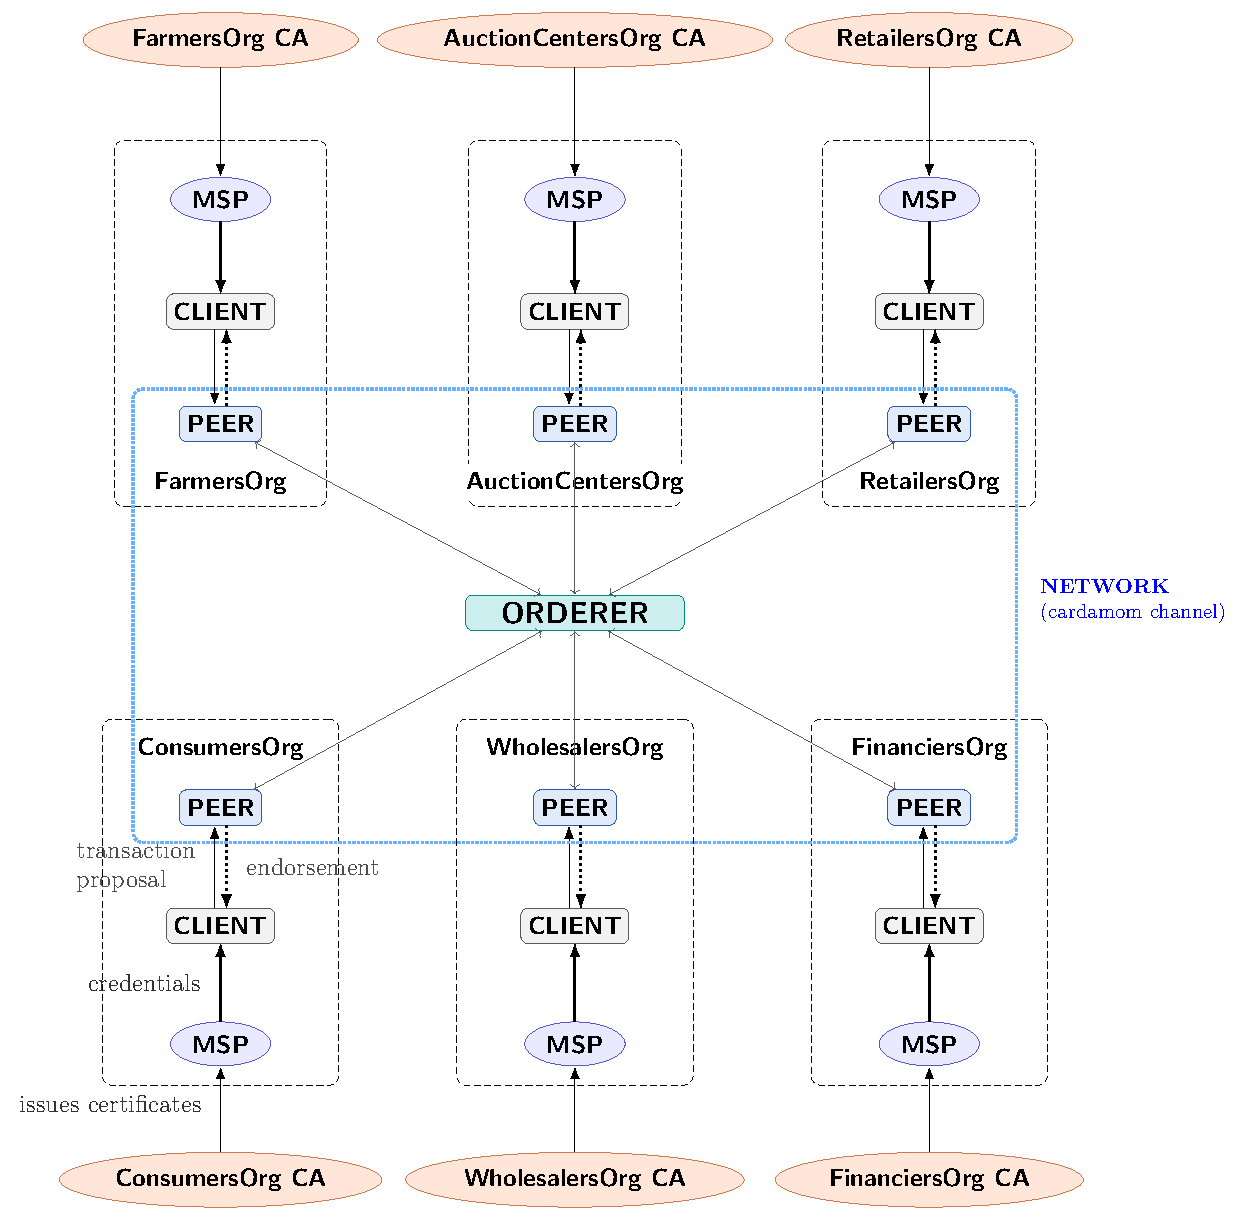
\includegraphics[width=\linewidth]{Figure_2.pdf}
		\caption{Blockchain network architecture showing participating organizations—Farmers, Auction Centers, Wholesalers, Consumers, and Financiers—connected through the \textit{cardamom channel}.}
		\label{fig:cardamom-network}
	\end{figure}
	
	
	\subsection{Smart Contract Workflow}
	
	The smart contract architecture is designed as a unified Hyperledger Fabric chaincode that orchestrates all transactions across the cardamom supply chain. 
	The architecture connects five major stakeholders, each represented as an independent organization within the Fabric network. 
	
	
	Each stakeholder interacts with the decentralized ledger via role-restricted functions enforced by MSP-based access control.
	All state updates—produce submission, bids, finance decisions, payments, grading results—are immutably stored and auditable.
	Events emitted by the chaincode enable real-time dashboard updates for auctions, finance decisions, and packet sales.
	
	Although implemented as a single contract, the logic is organized into functional segments that correspond to real-world operations: produce submission, quality testing, auction execution, financing, settlement, packet packing, packet sale, and audit queries.
	
	
	\subsubsection{Produce Submission and Quality Testing}
	The workflow begins when farmers invoke the \texttt{submitProduce()} function to submit their harvested produce to the approved auction centers along with key details like the weight of the produce, date of submission, number of bags, and the selected auction center. While submitting the testing fee gets deducted from the farmer's wallet, it is transferred to the auction center's wallet. All the details regarding the submission are immutably stored in the ledger for traceability. The testing fee is set by the auction center using \texttt{setTestingFee()}. The submitted produce undergoes rigorous testing by the auction center, which tests for pesticide limits above the maximum pesticide limit (MRL) and grades them depending on the size, color, and liter weight of the produce, and the metadata is recorded in the ledger by invoking the function \texttt{testCardamom()}. The workflow is illustrated in Fig.~\ref{fig:produce-auction-workflow}.
	
	
	
	\subsubsection{Auction Mechanism}
	
	Once the requisite tests are complete, the auction center lists the approved lots for auction with specified terms like bid increment and reserve price using the \texttt{openAuction()} function. After the auction is opened, the wholesalers make bids using the \texttt{placeBid()} function. Once the bid time prescribed by the auction center is closed, the auction center closes the bidding process by invoking \texttt{closeAuction()}. The chaincode then records the highest eligible offer, which can be inspected through \texttt{getHighestOfferForLot()} or \texttt{getBestOfferForAuction()}. Once the auction is closed, the farmers can review the bid offers using \texttt{farmerReviewBidForLot()}. In case of rejection by the farmer, the bid process is repeated. If accepted, the wholesalers can pay from their own wallet or can request finance from the financier. 
	
	\begin{figure}[!ht]
		\centering
		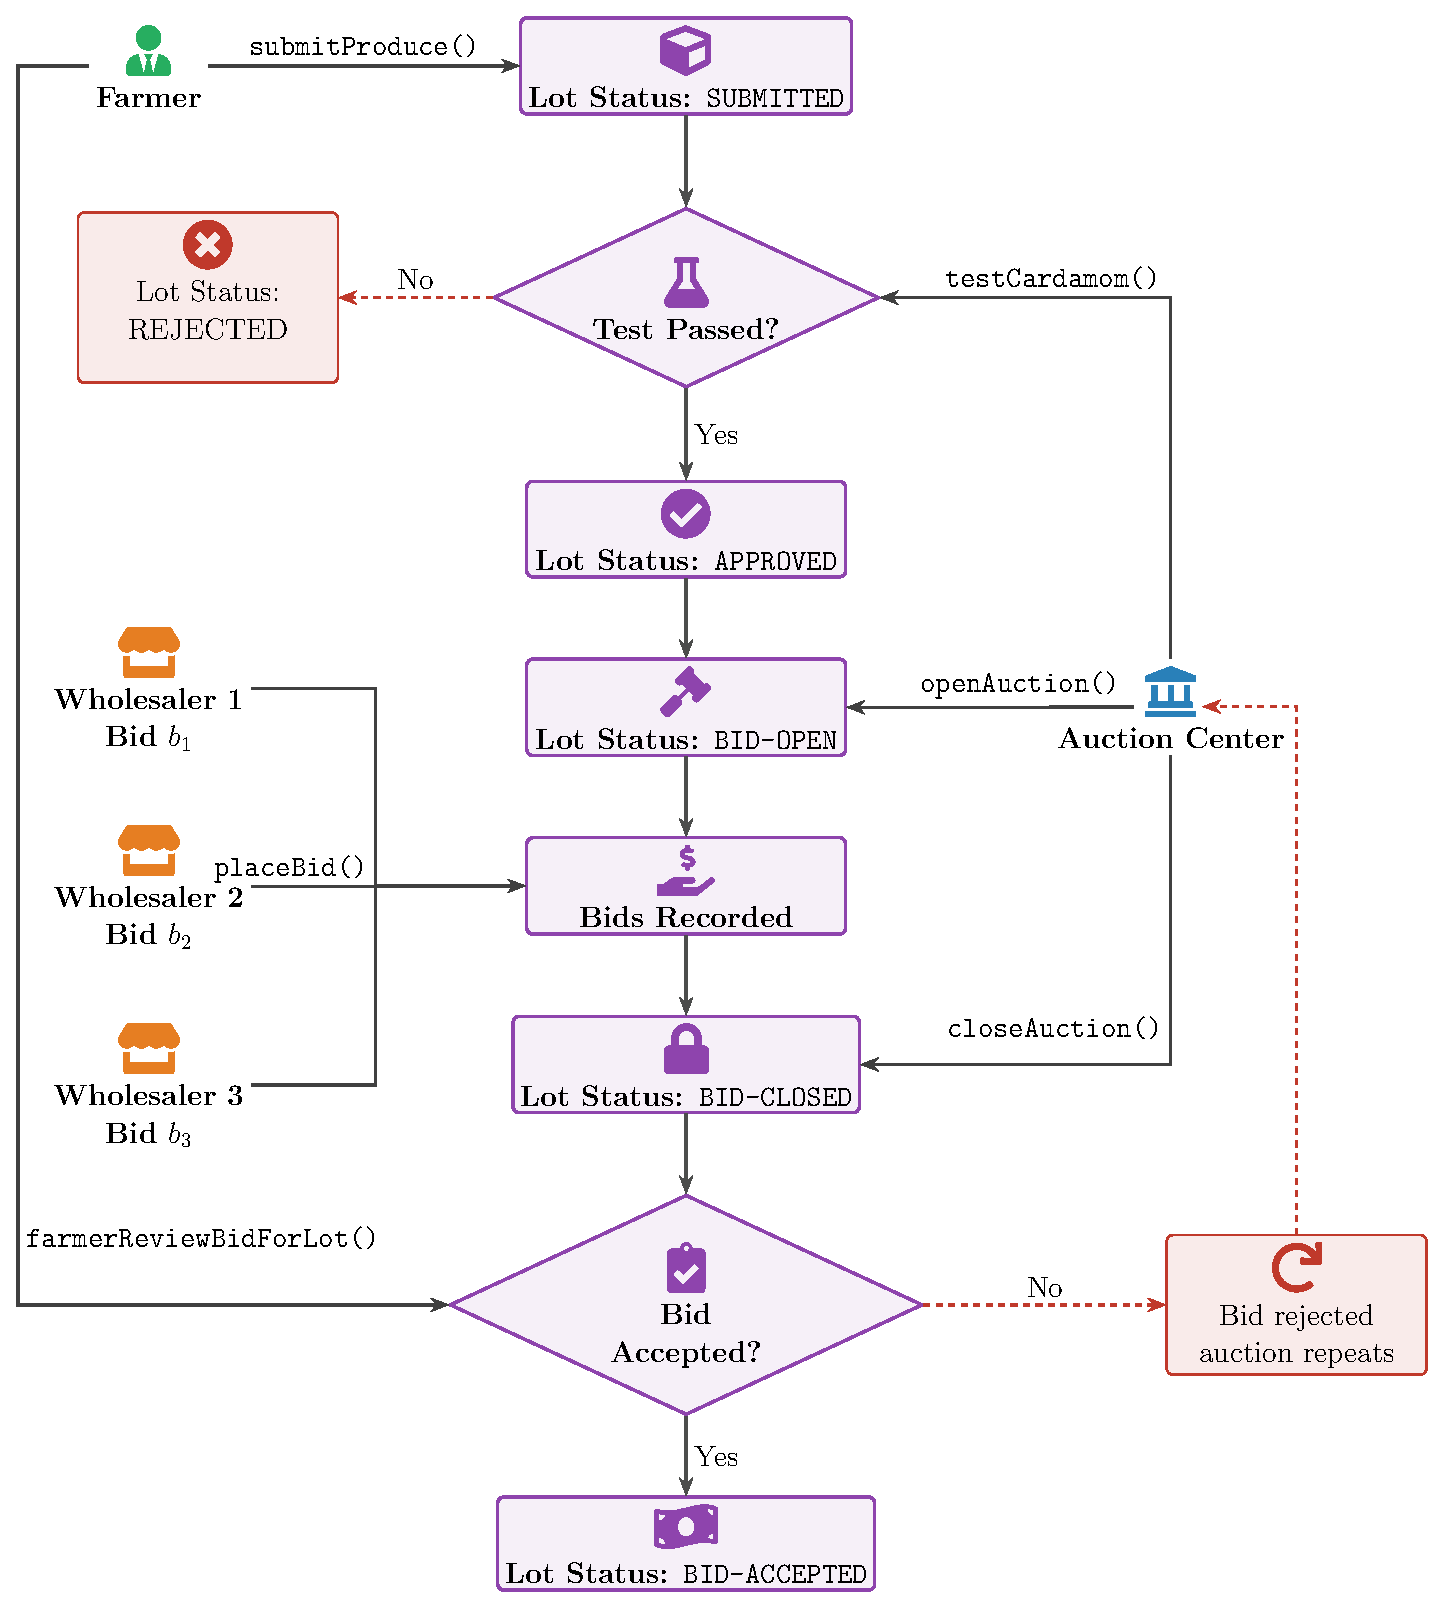
\includegraphics[width=\linewidth,height=0.82\textheight,keepaspectratio]{Figure_3.pdf}
		\caption{Produce submission and auction mechanism with quality testing, bid review, and multiple wholesalers}
		\label{fig:produce-auction-workflow}
	\end{figure}
	
	
	
	\subsubsection{Financing Workflow}
	
	After the auction is closed and the farmer accepts the winning bid, the winning wholesaler can either settle the lot from its own wallet or request finance from a financier. In the self-payment path, the accepted bid amount is directly transferred from the wholesaler's wallet to the farmer's wallet during the farmer-review stage. In the finance path, the lot status is updated to \texttt{BID-ACCEPTED}, allowing the wholesaler to initiate financing.
	
	The wholesaler first queries available finance offers from different financiers using an off-chain service to request APR rates. Since financiers may adopt different APR-setting strategies, the returned offers can include both fixed-interest quotations and adaptive quotations. Fixed-interest financiers quote a predefined APR, while RL-based financiers estimate APRs from historical finance-request records stored on the ledger, including principal, APR, tenor, fee, repayment, overdue status, outstanding amount, and realised profit values. The policy limits and quotation metadata are reflected on chain through finance-policy and RL-offer functions. These loan-level outcomes allow adaptive financiers to revise future APR quotations according to past lending performance.
	
	After comparing the available APRs and terms, the wholesaler selects a financier and invokes \texttt{createFinanceRequestForLot()}. This function verifies the accepted lot, confirms the closed auction, checks that the caller is the winning bidder, derives the principal from the highest bid, and stores a \texttt{PENDING} finance request on the ledger.
	
	The selected financier reviews the request using \texttt{reviewFinanceRequest()}; the variant \texttt{approveFinanceRequestWithAPR()} supports approval with an explicitly supplied APR. If approved, the smart contract computes the fee, interest, total payable amount, and outstanding liability. The internal function \texttt{\_disburseApprovedFinanceForLot()} is then executed automatically, debiting the financier's wallet and transferring the net amount to the farmer after deducting the nominal fee. The finance request is updated to \texttt{DISBURSED}, the repayment due date is recorded, the lot is marked as sold, and the payment record is stored on the ledger. Incoming and historical finance records can then be inspected through finance-query functions. This end-to-end process is illustrated in Fig.~\ref{fig:finance-offer-flowchart}.
	
	\begin{figure}[!ht]
		\centering
		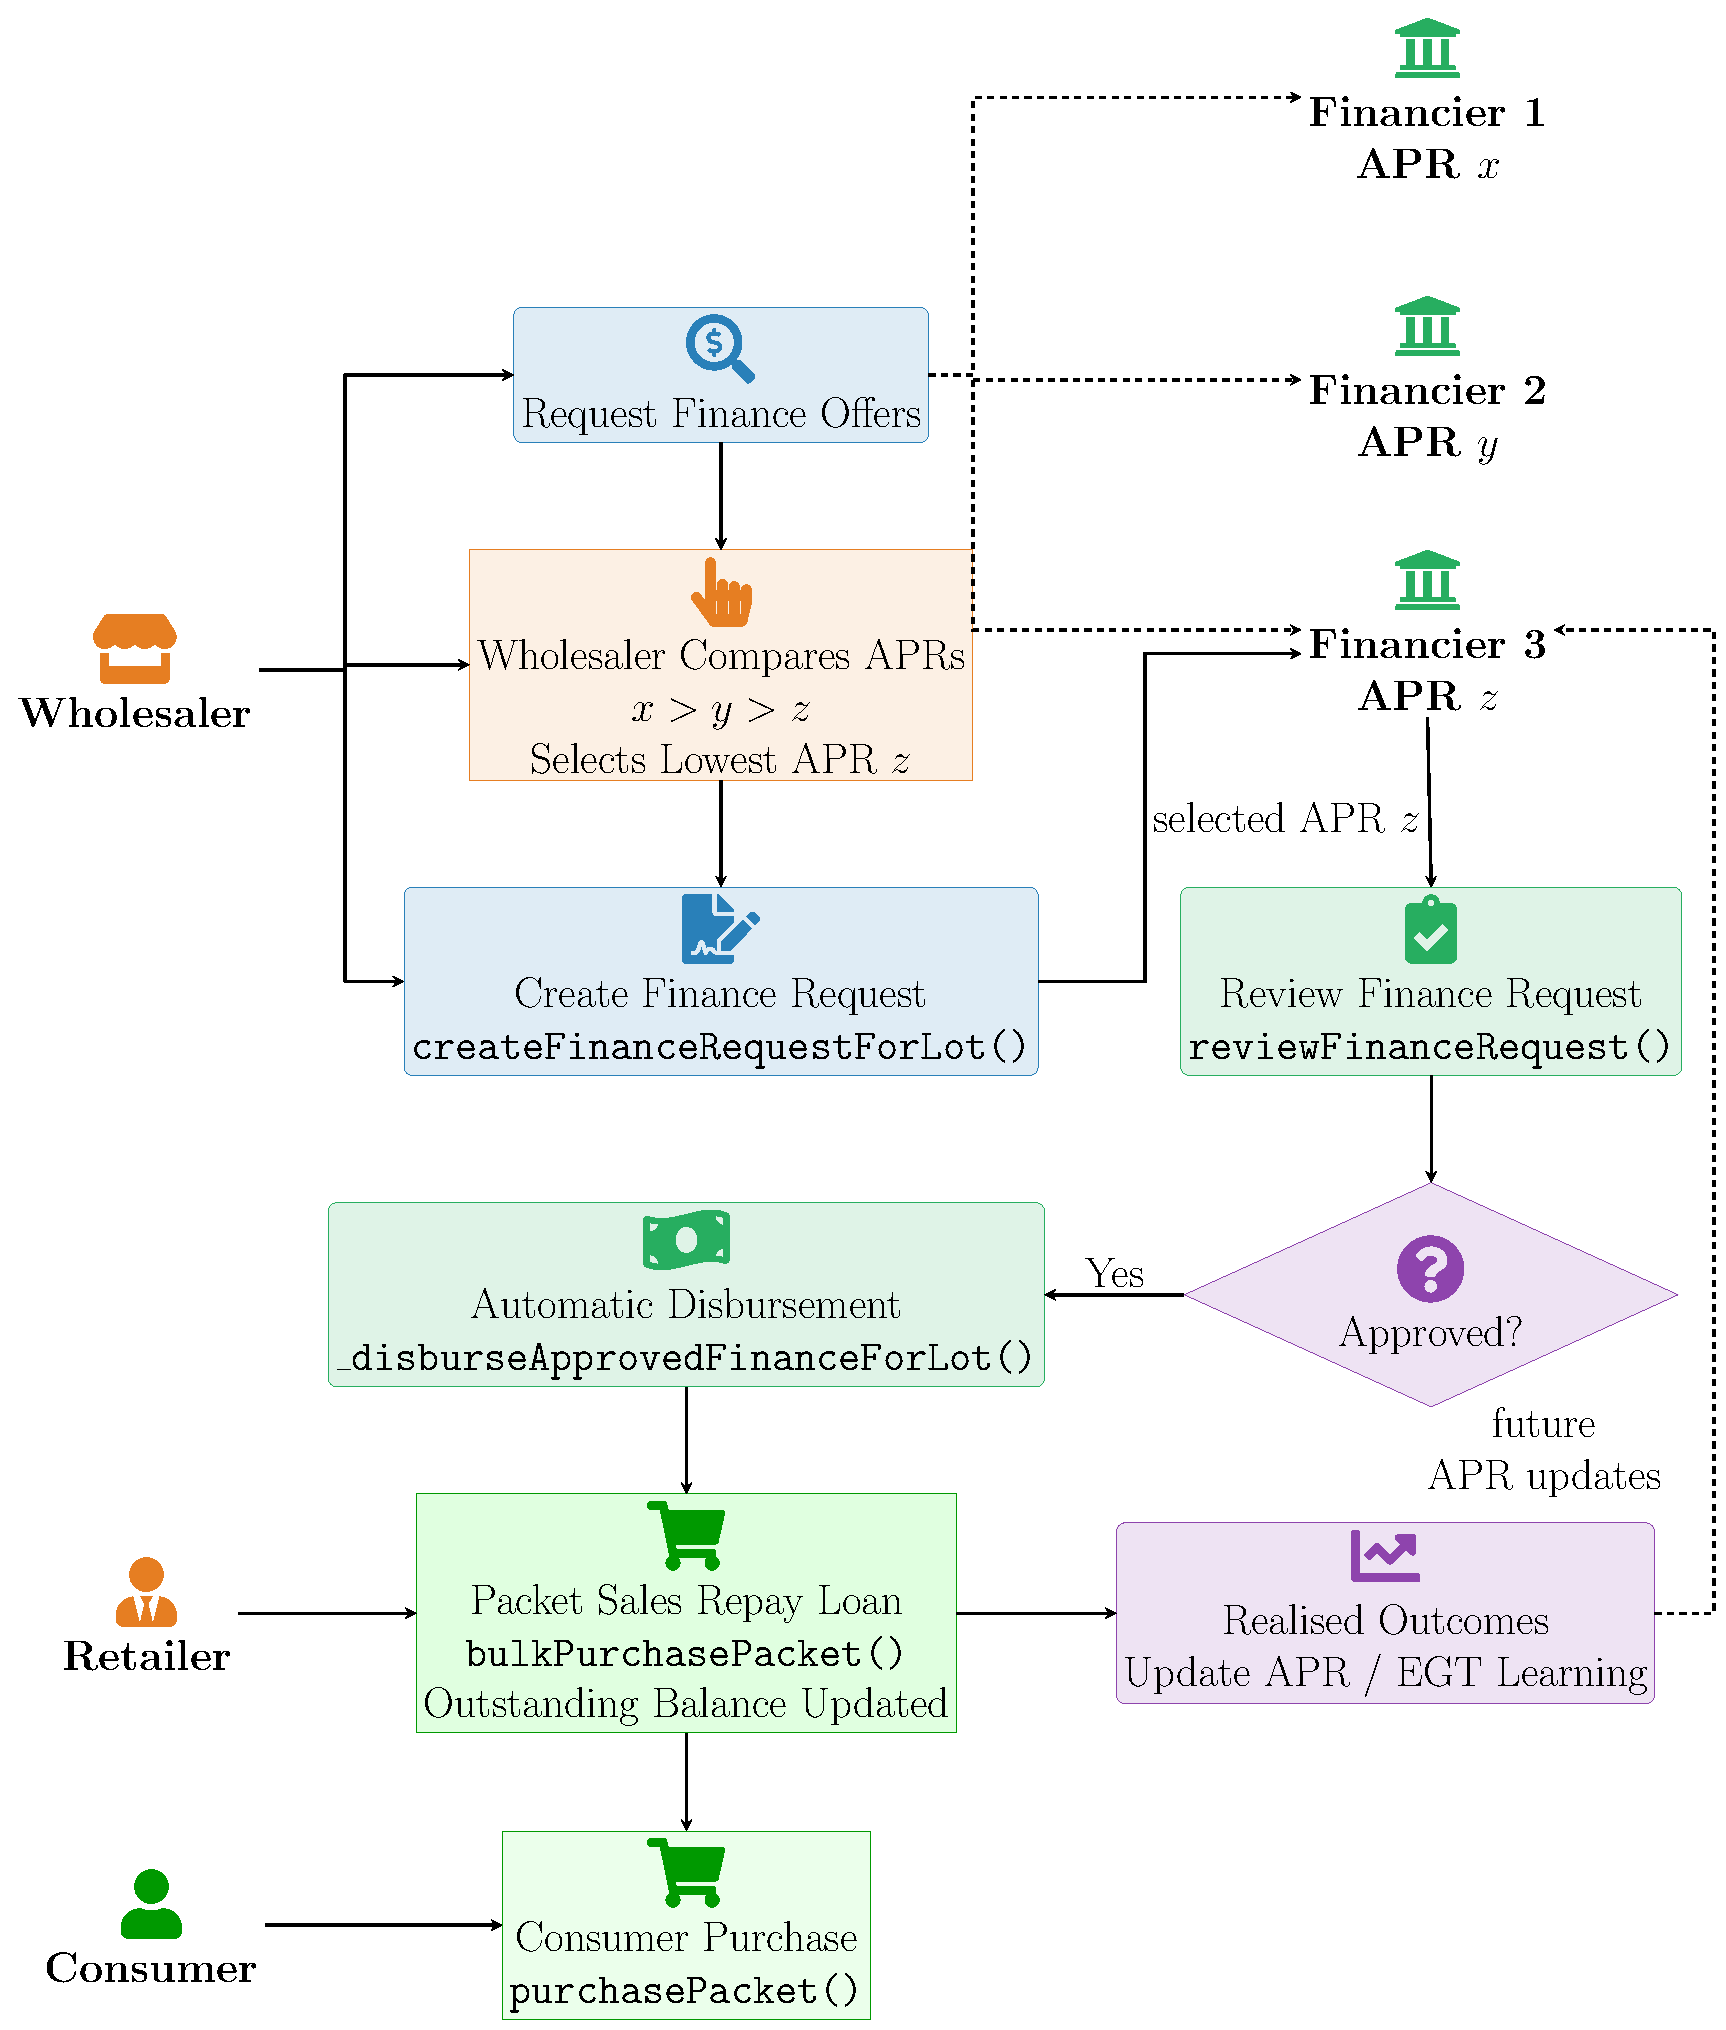
\includegraphics[width=\textwidth,height=0.82\textheight,keepaspectratio]{Figure_4.pdf}
		\caption{Finance-offer workflow with multiple financiers, APR comparison, finance-request creation, and financier approval}
		\label{fig:finance-offer-flowchart}
	\end{figure}
	
	After packet sale and loan settlement, the finance-request record is updated with repayment, outstanding balance, overdue status, financier profit, and wholesaler profit. These realised outcomes are used by the adaptive learning mechanism to influence future APR offers and credit terms. The score-oriented query functions \texttt{getWholesalerScore()} and \texttt{getFinancierScore()} expose the ledger-derived behavioural summaries used for monitoring and decision support.
	
	
	
	
	
	\subsubsection{Packet Packing and Consumer Sale}
	
	After auction settlement, ownership of the lot is transferred to the winning wholesaler. If the lot is self-funded, the wholesaler pays the farmer directly. If finance is used, the approved finance amount is disbursed from the financier's wallet to the farmer's wallet after deducting the nominal fee.
	
	Once the lot is marked as \texttt{SOLD}, the wholesaler invokes \texttt{packLotIntoPackets()} to divide the lot into packets. In this function, the wholesaler specifies the packet sizes, distribution percentages, and initial wholesale packet prices. Each packet is assigned a unique identifier and linked to the original lot, enabling provenance tracking from the consumer packet back to the farmer, auction, quality-testing record, and finance request. The wholesale price can later be updated by weight category using \texttt{setPacketPriceForWeight()}.
	
Retailers purchase available packets in bulk from wholesalers. The smart contract verifies the retailer, checks packet availability, reads the wholesale packet price, and transfers payment from the retailer wallet to the wholesaler. If the lot is financed, the wholesale packet-sale proceeds are first routed to the financier until the outstanding amount is repaid; any remaining proceeds are retained by the wholesaler. After this transaction, packet ownership is transferred to the retailer, and the packet status is updated to \texttt{AVAILABLE\_FOR\_CONSUMER\_PURCHASE}.

In the next layer, retailers set the consumer-facing packet price, and consumers purchase packets from retailers. The smart contract verifies the consumer, checks that the packet is available for consumer sale, reads the retailer-fixed selling price, and transfers payment from the consumer wallet to the retailer wallet. After successful purchase, packet ownership is transferred to the consumer, and the packet status is updated to \texttt{PURCHASED}. Packet-level audit trails are available through query functions.
	
	The finance request linked to the lot is updated with repayment, outstanding balance, overdue status, settlement date, and realised profit values. Once all packets of the financed lot are sold, these realised outcomes become available for adaptive learning and are used to influence future APR quotations and credit terms.
	
	
	
	
	\subsubsection{Wallet Management}
	
	In the supply chain, each participant maintains a digital wallet issued by the Financiers' organization. The system employs a token-based internal currency that is pegged against the Indian rupee. Real fiat money is converted to tokens and deposited into participants' digital wallets by authorised financiers, who act as on-chain liquidity providers. Tokens can be deposited by invoking the \texttt{depositMoney()} function, and token transfer occurs through the \texttt{transferMoney()} function.
	

	\subsection{Adaptive finance mechanism: RL-based APR optimisation and federated RL borrower screening}
	
	The APR offered to a wholesaler is determined through a two-stage mechanism. In the first stage, each financier determines a base APR according to its selected finance strategy. Different financiers may follow different strategies, including fixed-interest policies, RL-based adaptive APR policies, or other learning-based variants. For RL-based financiers, the base APR is estimated using portfolio-level signals such as capital utilisation and realised financier payoff. This stage captures the financier's macro-level lending condition and adjusts the baseline rate according to liquidity pressure and historical return.
	
	In the second stage, a borrower-specific adjustment is applied using the wholesaler's past finance-request history. This includes repayment performance, overdue behaviour, realised wholesaler profit, and prior loan outcomes. The borrower-side adjustment modifies the base APR by adding a risk premium or discount depending on the wholesaler's observed behaviour. Therefore, the final offered APR is expressed as:
	
	\[
	\mathrm{APR}^{\mathrm{offer}}
	=
	\mathrm{APR}^{\mathrm{base}}_{\mathrm{strategy}}
	+
	\mathrm{RiskPremium}_{\mathrm{wholesaler}}.
	\]
	
	The resulting APR is constrained within the minimum and maximum limits defined for the financier's policy. Thus, the APR offered to the wholesaler may be static or adaptive depending on the strategy used by the financier. The learning computation, where applicable, is performed outside the chaincode, and only the resulting finance offer is passed to the blockchain workflow.
	
	The performance of these alternative finance strategies is evaluated in the following experimental section. The best-performing strategy is selected based on comparative simulation results against fixed-interest baseline models and learning-based variants.

	
\subsection{Blockchain Integration of Selected Finance Policy}

After the simulation-based model selection, the selected finance policy was connected to the blockchain framework through the backend service rather than being embedded directly inside the smart contract. The adaptive APR decision is computed by an off-chain Python service, which evaluates the financier-side APR strategy and borrower-side screening output using simulation-derived policy logic. The wholesaler accesses the offered APR through the backend application and compares the finance terms made available by financiers. Based on these displayed terms, the wholesaler can select a financier and create a finance request for the accepted cardamom lot.

The blockchain smart contract is used to record and enforce the resulting finance workflow after the wholesaler initiates the request. Once a wholesaler wins an auction and the farmer accepts the bid, the wholesaler can either pay the farmer directly from its wallet or request finance from a selected financier. In the finance-request path, the ledger records the lot identifier, wholesaler identifier, financier identifier, principal amount, APR, fee, penalty, tenor, outstanding amount, repayment status, and settlement history. Thus, the adaptive finance policy operates as an off-chain decision-support layer, while the blockchain layer provides transaction recording, access control, settlement execution, and traceability.

This design separates computational intelligence from ledger execution. The Python backend service performs the APR recommendation and finance-policy evaluation, while Hyperledger Fabric stores the accepted finance terms and executes the approved transaction flow. When finance is approved, the smart contract disburses the financed amount to the farmer, records the repayment obligation of the wholesaler, and updates the finance request during packet sales and repayment events. This creates an auditable finance trail covering finance request creation, approval, disbursement, repayment, overdue calculation, settlement, and transaction history.

By linking the off-chain RL--FL finance policy with the on-chain transaction workflow, the proposed framework supports risk-aware supply chain finance without overloading the smart contract with learning logic. The ledger stores operational events such as produce submission, testing, auction, packing, and packet purchase, along with authorised financial events such as finance request creation, approval, repayment, and settlement. Each finance decision can therefore be traced to the corresponding cardamom lot and auction outcome by authorised participants, while raw client learning records remain under the control of the originating financier.

For federated borrower screening, the blockchain is used as a permissioned coordination and audit layer for Q-table aggregation rather than as a shared repository of borrower records. Each financier trains its borrower-screening Q-table locally and submits only the model-level state--action Q-values for a federation round. This workflow is supported by three chaincode operations: \texttt{submitFederatedQUpdate()} records an authorised financier's Q-table update for a specific round, \texttt{aggregateFederatedQTables()} computes or finalises the round-level averaged Q-table from submitted updates, and \texttt{getFederatedQTable()} allows authorised financiers to retrieve the approved aggregated Q-table version. The resulting model can then be used by the backend to generate finance offers through the existing finance-policy workflow. The ledger stores Q-value parameters, aggregation-round identifiers, model-version metadata, timestamps, and update events, while raw borrower identities, individual repayment histories, account balances, and complete transaction records remain with the originating financier.
	
	\subsection{Experimental Design for Finance Model Selection}
	
	\subsubsection{Simulation Setup and Agents}
	
	A discrete-event simulation evaluates the finance-offer models across varying capital constraints, default scenarios, and random seeds. The environment abstracts the physical supply chain to focus purely on financial interactions: loan requests, APR quotations, repayment, and defaults. The simulation features two primary agents:
	\begin{itemize}
		\item \textbf{Financiers} determine a base APR bounded between 6\% and 36\%. They employ either fixed-rate strategies (6\%, 8\%, 10\%) or a reinforcement-learning (RL) strategy that adapts based on portfolio utilisation and loan outcomes.
		\item \textbf{Wholesalers} seek financing and select the most competitive APR offer. The system applies isolated or federated RL borrower screening to assign a borrower-specific risk premium (between \(-2\%\) and \(16\%\)) from locally held repayment and profitability signals.
	\end{itemize}
	The experiment evaluates combinations of these financier and borrower-side strategies (Table~\ref{tab:basic-finance-strategy-combinations}).
	
	\begin{table}[h]
		\centering
		\caption{Basic finance-strategy combinations}
		\label{tab:basic-finance-strategy-combinations}
		\begin{tabular}{|C{0.28\linewidth}|C{0.32\linewidth}|C{0.28\linewidth}|}
			\hline
			\textbf{Financier-side APR strategy} & \textbf{Borrower-side screening strategy} & \textbf{Combination} \\
			\hline
			RL APR & RL borrower screening & RL + RL \\
			\hline
			RL APR & FL RL borrower screening & RL + FL RL \\
			\hline
			RL APR & No borrower screening & RL + none \\
			\hline
			Fixed APR & No borrower screening & Fixed + none \\
			\hline
		\end{tabular}
	\end{table}
	
	\subsubsection{Reinforcement Learning Formulation}
	
	Tabular Q-learning is selected for the adaptive finance models due to its computational efficiency, exact policy capture over small discrete state spaces, and full interpretability—critical for financial auditing. Unlike deep reinforcement learning methods that rely on black-box function approximators, Q-tables explicitly map every state-action pair to an expected reward, ensuring that finance-offer decisions remain transparent and predictable. RL is applied at two independent levels to distinguish portfolio-level adaptation from borrower-level screening: the financier-side RL agent sets the base APR, and the borrower-side RL agent determines the risk premium. Both models use an \(\epsilon\)-greedy action-selection rule and update their respective Q-tables using the standard Bellman equation:
	\[
	Q(s_t, a_t) \leftarrow Q(s_t, a_t) + \alpha \left[ r_t + \gamma \max_{a} Q(s_{t+1}, a) - Q(s_t, a_t) \right]
	\]
	where \(s_t\) is the current state, \(a_t\) is the selected action, \(r_t\) is the observed reward, \(\alpha\) is the learning rate, and \(\gamma\) is the discount factor.
	
	\paragraph{Financier-Side APR Learning}
	The financier-side RL problem is formulated as a portfolio-level base-APR optimisation problem. It observes only aggregate capital utilisation and selects a common base APR before borrower-specific screening is applied. The state, action, reward, and objective are defined as:
	\[
	\begin{aligned}
	s_t^{APR} &= \Phi\left(\frac{C^{deployed}_t}{C^{total}_t}\right),\\
	a_t^{APR} &\in \mathcal{A}^{APR}=\{6,7,\ldots,36\},\\
	r_t^{APR} &\in \{r_t^{projected},r_t^{realised}\},\\
	\pi^{APR*} &= \arg\max_{\pi^{APR}}\mathrm{E}\left[\sum_{t=0}^{T}\gamma^{t}r_t^{APR}\right].
	\end{aligned}
	\]
	Here, \(s_t^{APR}\) is the discretised capital-utilisation state, \(a_t^{APR}\) is the selected base APR, and \(\pi^{APR*}\) is the learned APR policy. The reward is portfolio-facing and is implemented in two steps. At loan issuance, the agent receives a projected reward based on the expected interest from the offered APR:
	
	\[
	\begin{aligned}
	\mathrm{ProjectedInterest}_t
	&= \mathrm{Principal}_t \times \mathrm{APR}^{base}_t \times \frac{\mathrm{Tenor}_t}{365},\\
	r_t^{projected}
	&= \mathrm{clip}\left(\frac{\mathrm{ProjectedInterest}_t}{\max(1,\mathrm{Principal}_t)},-1,1\right).
	\end{aligned}
	\]
	When the loan is closed, this provisional signal is corrected using the realised repayment outcome:
	\[
	\begin{aligned}
	y_t
	&=
	\frac{
		\mathrm{InterestPaid}_t+\mathrm{PenaltyPaid}_t-\mathrm{DefaultAmount}_t
	}{
		\max(1,\mathrm{Principal}_t)
	},\\
	r_t^{realised}
	&= \mathrm{clip}\left(\frac{y_t}{1+|y_t|},-1,1\right).
	\end{aligned}
	\]
	This projected-then-realised reward structure is used because the final loan outcome is observed only after sale and settlement. The projected reward gives the Q-learning agent an immediate learning signal when the finance offer is issued, while the realised correction prevents the policy from over-rewarding offers that later experience overdue repayment or default.
	
	\paragraph{Borrower-Side Screening and Final APR}
	
	Borrower-side screening dynamically assigns a risk premium based on wholesaler repayment history. The simulation subjects 39 wholesalers to varying levels of repayment stress (Table~\ref{tab:wholesaler-risk-profile-composition}). The system evaluates two adaptive screening methods:
	
	\textbf{RL Screening:} In contrast, the borrower-side RL screening model is a borrower-level risk-premium optimisation problem. For each borrower \(i\), the state is based on an exponentially smoothed net-profit ratio:
	\[
	\mathrm{EWMAProfitRatio}_{i,t} =
	\begin{cases}
		\pi_{i,t}, & t=1,\\
		0.8\,\mathrm{EWMAProfitRatio}_{i,t-1} + 0.2\,\pi_{i,t}, & t>1.
	\end{cases}
	\]
	The corresponding RL components are:
	\[
	\begin{aligned}
	s_{i,t}^{RP} &= \Psi\left(\mathrm{EWMAProfitRatio}_{i,t}\right),\\
	a_{i,t}^{RP} &\in \mathcal{A}^{RP}=\{-2,0,4,8,12,16\},\\
	r_{i,t}^{RP} &= \pi_{i,t}-\lambda I(\mathrm{default}_{i,t}),\\
	\pi^{RP*} &= \arg\max_{\pi^{RP}}\mathrm{E}\left[\sum_{t=0}^{T}\gamma^{t}r_{i,t}^{RP}\right].
	\end{aligned}
	\]
	Here, \(\Psi\) discretises individual borrower performance, \(a_{i,t}^{RP}\) is the borrower-specific risk premium, \(\lambda\) is the default penalty factor, and \(I(\mathrm{default}_{i,t})\) is an indicator for borrower \(i\)'s default. Unlike the financier-side APR learner, this agent does not choose the portfolio base rate; it adjusts the borrower-specific premium added to that base rate.
	
	\textbf{Federated RL Screening:} The borrower-side RL model can operate in isolated or federated mode. In isolated mode, each financier updates only its local borrower Q-table. In FL-RL mode, each financier submits its learned state--action Q-values to the permissioned blockchain for the current aggregation round. The smart contract accepts updates only from authorised financiers, stores the submitted model parameters by round and financier, averages corresponding Q-values across valid submissions, and publishes the approved aggregated Q-table version for retrieval by participating financiers. The local borrower records used to train those Q-values are not submitted. Raw client records, borrower identities, individual repayment histories, account balances, and complete transaction records are therefore not transferred as training data. This permits blockchain-mediated Q-table aggregation while retaining source records locally. Because Q-values can still reveal information under some attacks, the design is described as privacy-conscious rather than as providing formal cryptographic privacy.

	\textbf{Final APR Calculation:} The final offered APR combines the financier base APR and the RL borrower risk premium, strictly bounded between 6\% and 36\%:
	\[
	\mathrm{APR}^{offer}_t
	= \mathrm{clip}
	\left(
	\mathrm{APR}^{base}_t + \mathrm{RiskPremium}_t,
	6\%,
	36\%
	\right).
	\]
	
	\begin{table}[h]
		\centering
		\caption{Wholesaler risk-profile composition used in the simulation}
		\label{tab:wholesaler-risk-profile-composition}
		\begin{tabular}{|C{0.28\linewidth}|c|c|c|c|}
			\hline
			\textbf{Default scenario} & \textbf{Total wholesalers} & \textbf{No-shock} & \textbf{Medium-shock} & \textbf{High-shock} \\
			\hline
			No-default & 39 & 39 & 0 & 0 \\
			\hline
			Low-default & 39 & 34 & 4 & 1 \\
			\hline
			Medium-default & 39 & 30 & 7 & 2 \\
			\hline
			High-default & 39 & 25 & 10 & 4 \\
			\hline
		\end{tabular}
	\end{table}
	
	\subsubsection{Experimental Design and Staged Evaluation}
	
	The experiment employs a staged model-selection pipeline to isolate and optimise the financier-side and borrower-side learning mechanisms sequentially. The earlier hyperparameter-selection stage uses 36 runs spanning three initial-capital levels (1~M, 5~M, and 10~M), four default profiles, and three random seeds. The subsequent federated-versus-isolated RL ablation is reported separately over four complete seeds (944649, 709098, 436570, and 831197), covering 48 matched combinations of three capital levels and four default profiles across a 4000-day horizon. The default profiles progressively reduce the realised gross margins of affected wholesalers (from a 20\% base margin down to as low as \(-12\%\)), thereby increasing repayment stress and the probability of default.
	
	The evaluation proceeds in three stages:
	\begin{enumerate}
		\item \textbf{Stage 1: Financier-Side APR Optimisation.} Isolates the RL base-APR learner (without borrower screening) against fixed-rate 6\%, 8\%, and 10\% baselines. 
		\item \textbf{Stage 2: Borrower-Side RL Optimisation.} Tunes the isolated borrower-screening RL learner across its learning rate, discount factor, exploration rate, and risk-premium action grid.
		\item \textbf{Stage 3: Federated RL Ablation.} Compares FL-RL with isolated RL screening across four seeds and the 12 combinations of three initial-capital levels and four default-severity profiles. Return on initial capital, net profit, and loan-count default rate are compared within each matched scenario.
	\end{enumerate}
	
	Table~\ref{tab:combined-hyperparameter-grids} summarises the parameter search spaces used in the respective optimisation stages.
	
	\begin{table}[h]
		\centering
		\caption{Hyperparameter optimisation grids for the RL components}
		\label{tab:combined-hyperparameter-grids}
		\begin{tabular}{|C{0.23\linewidth}|C{0.67\linewidth}|}
			\hline
			\textbf{Component} & \textbf{Parameters Tested} \\
			\hline
			Financier RL APR & \(\alpha_{APR} \in \{0.1, 0.25, 0.4\}\), \(\gamma_{APR} \in \{0.5, 0.7, 0.95\}\), \(\epsilon_{APR} \in \{0.02, 0.05, 0.08\}\), \newline Action grid: 1\%, 2\%, or 3\% steps from 6\% to 36\% \\
			\hline
			Borrower RL Screening & \(\alpha_{B} \in \{0.1, 0.25, 0.4\}\), \(\gamma_{B} \in \{0.5, 0.7, 0.95\}\), \(\epsilon_{B} \in \{0.02, 0.05, 0.12\}\), \newline Action grid: Coarse ($\{-2, 0, 4, 8, 12, 16\}$), Fine ($\{-2, 0, 2, \dots, 16\}$), or Hybrid ($\{-2, 0, 2, 4, 8, 12, 16\}$) \\
			\hline
		\end{tabular}
	\end{table}

\subsubsection{Sensitivity Analysis Setup}

After selecting the RL base-APR and borrower-screening parameters, a matched federated sensitivity analysis was conducted across multiple initial-capital levels and default-severity conditions. FL-RL and isolated RL used the same seed, capital, repayment-stress profile, and 4000-day horizon in each comparison. The models were evaluated over the 1M, 5M, and 10M capital levels under no-default, low-default, medium-default, and high-default conditions, repeated over four complete seeds.

	
	
	\subsection{Blockchain Benchmarking Setup}
	
	The performance of the proposed Hyperledger Fabric network was evaluated using Hyperledger Caliper. To emulate concurrent client-side interactions, the benchmark was configured with five parallel workers submitting transactions through the Fabric Gateway. The evaluation tested the primary smart contract functions—including lot submission, quality testing, auction bidding, finance operations, packet creation, and purchase—capturing both lightweight queries and state-intensive updates. For each workload, Caliper recorded standard metrics: transaction throughput (successful ledger commits per second), latency (time from submission to confirmation), and the total count of successful and failed transactions. This setup enables a comparative assessment of the network's processing capacity and responsiveness under load.
	

	

	
	\section{Results and Discussion}

	\subsection{Validation of Auction, Finance, and Settlement Workflow}
	
	The proposed Hyperledger Fabric smart contract was validated by executing the complete cardamom supply chain finance workflow from produce submission to final sale settlement. The execution confirmed that the contract enforces a strict state-transition sequence covering produce submission, quality testing, auction opening, bid placement, farmer review, finance approval, packet creation, purchase, and repayment. Out-of-order operations, such as opening an auction before quality approval or initiating finance before farmer acceptance, were rejected by the contract logic. This confirms that the workflow is not merely recorded on the blockchain but is actively governed by smart-contract rules.
	
	The auction workflow demonstrated that every lot submission, test result, bid, auction decision, and ownership update was immutably recorded on the ledger. This prevents repeated or unauthorised rebidding of the same lot and creates a tamper-evident audit trail that can be verified by authorised network participants. The farmer-review stage was particularly important because it allowed the farmer to accept or reject the highest bid before the lot advanced to payment or financing. Thus, the proposed system addresses a major limitation of traditional cardamom auction practices, where farmers often have limited control over post-auction settlement decisions.
	
	The finance and settlement workflow also executed as intended. After farmer acceptance, the winning wholesaler could either settle the lot directly from its wallet or request finance from a financier. In the financed case, the smart contract created the finance request, enabled financier review, disbursed the approved amount to the farmer, and recorded the outstanding repayment obligation on the ledger. During subsequent packet purchase, the contract automatically routed sale proceeds toward loan repayment before transferring any remaining amount to the wholesaler. This shows that repayment is embedded into the sale transaction itself rather than being handled as a separate manual process. As a result, the workflow reduces settlement delay for farmers, improves repayment assurance for financiers, and increases transparency across the auction-finance-sale cycle.

\subsection{Finance Model Selection and Parameter Optimisation}

The results are reported in three steps: financier-side base-APR optimisation, borrower-side RL parameter optimisation, and a matched federated ablation. This sequence isolates portfolio-level APR adaptation from borrower-level screening and then tests the marginal effect of federated aggregation against isolated RL.

\textbf{Stage 1: Financier-side base-APR optimisation.} The reinforcement learning (RL) base-APR learner was evaluated with borrower screening switched off and compared against fixed 6\%, 8\%, and 10\% APR baselines. As shown in Table~\ref{tab:financier-rl-optimization-results}, the RL-based APR optimiser achieved the highest final capital (254.39M) while maintaining a balanced default exposure (18.77\%) and utilisation (0.648), outperforming the static alternatives. Therefore, the RL-based APR optimiser was adopted as the financier-side base-APR mechanism for the subsequent stages.
	
\begin{table}[H]
	\centering
	\caption{Stage 1 financier-side base-APR optimisation results}
	\label{tab:financier-rl-optimization-results}
	\small
	\setlength{\tabcolsep}{2pt}
	\renewcommand{\arraystretch}{1.12}
	\begin{tabular}{|C{0.22\linewidth}|c|C{0.11\linewidth}|C{0.11\linewidth}|c|C{0.14\linewidth}|c|}
		\hline
		\textbf{Financier strategy} & \textbf{Runs} & \textbf{Initial capital} & \textbf{Final capital} & \textbf{Avg. APR} & \textbf{Default / initial capital} & \textbf{Avg. util.} \\
		\hline
		RL base-APR optimiser, no screening & 36 & 192M & 254.39M & 10.19\% & 18.77\% & 0.648 \\
		\hline
		Fixed 6\%, no screening & 36 & 192M & 234.73M & 6.00\% & 28.88\% & 0.809 \\
		\hline
		Fixed 10\%, no screening & 36 & 192M & 204.28M & 10.00\% & 3.31\% & 0.321 \\
		\hline
		Fixed 8\%, no screening & 36 & 192M & 201.35M & 8.00\% & 6.59\% & 0.376 \\
		\hline
	\end{tabular}
\end{table}


\textbf{Stage 2: Borrower-side RL parameter optimisation.} With the RL base-APR optimiser selected in Stage 1, the borrower-side RL screening model was tuned across its learning rate, discount factor, exploration rate, and risk-premium action grid. Table~\ref{tab:borrower-rl-optimization-results} reports the leading configurations. The best setting used \(\alpha_B=0.10\), \(\gamma_B=0.70\), \(\epsilon_B=0.05\), and the coarse risk-premium grid, producing a final capital of 243.59M.
	
\begin{table}[H]
	\centering
	\caption{Borrower-side RL screening parameter optimisation results}
	\label{tab:borrower-rl-optimization-results}
	\small
	\setlength{\tabcolsep}{1.8pt}
	\renewcommand{\arraystretch}{1.25}
	\begin{tabular}{|
			>{\centering\arraybackslash}m{0.095\linewidth}|
			>{\centering\arraybackslash}m{0.095\linewidth}|
			>{\centering\arraybackslash}m{0.12\linewidth}|
			>{\centering\arraybackslash}m{0.125\linewidth}|
			>{\centering\arraybackslash}m{0.065\linewidth}|
			>{\centering\arraybackslash}m{0.09\linewidth}|
			>{\centering\arraybackslash}m{0.095\linewidth}|
			>{\centering\arraybackslash}m{0.075\linewidth}|
			>{\centering\arraybackslash}m{0.12\linewidth}|
		}
		\hline
		\textbf{\makecell[c]{Learn-\\ing\\rate\\\(\alpha_B\)}} &
		\textbf{\makecell[c]{Dis-\\count\\factor\\\(\gamma_B\)}} &
		\textbf{\makecell[c]{Explo-\\ration\\rate\\\(\epsilon_B\)}} &
		\textbf{\makecell[c]{Risk-\\premium\\grid}} &
		\textbf{\makecell[c]{Runs}} &
		\textbf{\makecell[c]{Initial\\capital}} &
		\textbf{\makecell[c]{Final\\capital}} &
		\textbf{\makecell[c]{Avg.\\APR}} &
		\textbf{\makecell[c]{Default /\\initial\\capital}} \\
		\hline
		0.10 & 0.70 & 0.05 & $\{-2, \allowbreak 0, \allowbreak 4, \allowbreak 8, \allowbreak 12, \allowbreak 16\}$ & 36 & 192M & 243.59M & 11.22\% & 7.95\% \\
		\hline
		0.10 & 0.70 & 0.05 & $\{-2, \allowbreak 0, \allowbreak 2, \allowbreak 4, \allowbreak 8, \allowbreak 12, \allowbreak 16\}$ & 36 & 192M & 243.57M & 10.92\% & 9.24\% \\
		\hline
		0.10 & 0.70 & 0.02 & $\{-2, \allowbreak 0, \allowbreak 2, \allowbreak 4, \allowbreak 8, \allowbreak 12, \allowbreak 16\}$ & 36 & 192M & 242.68M & 11.36\% & 11.39\% \\
		\hline
		0.10 & 0.95 & 0.02 & $\{-2, \allowbreak 0, \allowbreak 4, \allowbreak 8, \allowbreak 12, \allowbreak 16\}$ & 36 & 192M & 242.57M & 10.96\% & 7.42\% \\
		\hline
	\end{tabular}
\end{table}
\subsubsection{Final Combined Performance and Scenario Analysis}

\textbf{Combined non-federated baselines.} Table~\ref{tab:stage4-final-results} retains the relevant RL and fixed-rate baselines used to contextualise the federated experiment. The tuned RL base-APR model with isolated RL borrower screening exceeded the RL model without screening and the fixed-rate alternatives in aggregate final capital, supporting the value of adaptive borrower-level pricing before federated aggregation is introduced.
	
\begin{table}[h]
	\centering
	\caption{Non-federated RL and fixed-rate baseline results}
	\label{tab:stage4-final-results}
	\footnotesize
	\setlength{\tabcolsep}{2pt}
	\renewcommand{\arraystretch}{1.25}
	\begin{tabular}{|
			>{\centering\arraybackslash}m{0.32\linewidth}|
			>{\centering\arraybackslash}m{0.06\linewidth}|
			>{\centering\arraybackslash}m{0.11\linewidth}|
			>{\centering\arraybackslash}m{0.11\linewidth}|
			>{\centering\arraybackslash}m{0.09\linewidth}|
			>{\centering\arraybackslash}m{0.14\linewidth}|
			>{\centering\arraybackslash}m{0.11\linewidth}|
		}
		\hline
		\textbf{\makecell[c]{Financier strategy}} &
		\textbf{\makecell[c]{Runs}} &
		\textbf{\makecell[c]{Initial\\capital}} &
		\textbf{\makecell[c]{Final\\capital}} &
		\textbf{\makecell[c]{Avg.\\APR}} &
		\textbf{\makecell[c]{Default /\\initial\\capital}} &
		\textbf{\makecell[c]{Avg.\\utilisation}} \\
		\hline
		Optimised RL APR + RL screening & 36 & 192M & 241.85M & 12.10\% & 2.44\% & 0.413 \\
		\hline
		Optimised RL APR + no screening & 36 & 192M & 227.30M & 9.83\% & 12.20\% & 0.476 \\
		\hline
		Fixed 10\% APR + no screening & 36 & 192M & 201.89M & 10.00\% & 3.55\% & 0.305 \\
		\hline
		Fixed 6\% APR + no screening & 36 & 192M & 196.87M & 6.00\% & 30.52\% & 0.664 \\
		\hline
		Fixed 8\% APR + no screening & 36 & 192M & 195.40M & 8.00\% & 6.82\% & 0.344 \\
		\hline
	\end{tabular}
\end{table}
\subsubsection{Federated versus Non-Federated Borrower Screening}

To isolate the effect of collaborative model aggregation, the federated screening variants were compared with matched non-federated counterparts over 48 seed--capital--default combinations using a 4000-day horizon. Table~\ref{tab:federated-scenario-sensitivity} reports the scenario-level sensitivity results averaged across the four seeds for each capital--default pair. Table~\ref{tab:federated-ablation} then summarises all matched observations as averages. FL-RL achieved a higher return than isolated RL in 45 of the 48 matched comparisons and never produced a higher mean loan-count default rate. Its mean return on initial capital was 41.08\%, compared with 32.81\% for isolated RL, representing an average improvement of 8.27 percentage points. The mean loan-count default rate was also 4.60 percentage points lower, and cumulative net profit across the 48 matched comparisons was approximately 8.09M higher. The largest mean return improvement occurred in the 1M medium-default scenario, while the 1M high-default scenario remained the most profitable stress case: FL-RL achieved a 139.53\% return and a 1.84\% default rate, whereas isolated RL achieved a 106.56\% return and a 9.12\% default rate.

\begin{table}[H]
	\centering
	\caption{Scenario-level federated sensitivity across capital and default profiles (mean across four seeds)}
	\label{tab:federated-scenario-sensitivity}
	\scriptsize
	\setlength{\tabcolsep}{2.5pt}
	\renewcommand{\arraystretch}{1.15}
	\resizebox{\textwidth}{!}{%
	\begin{tabular}{|c|l|c|c|c|c|c|c|}
		\hline
		\textbf{Capital} &
		\textbf{Default profile} &
		\textbf{\makecell[c]{FL-RL\\return}} &
		\textbf{\makecell[c]{Isolated RL\\return}} &
		\textbf{\(\Delta\) return} &
		\textbf{\makecell[c]{FL-RL\\default rate}} &
		\textbf{\makecell[c]{Isolated RL\\default rate}} &
		\textbf{\(\Delta\) default} \\
		\hline
		1M & None & 81.91\% & 79.91\% & +2.00 pp & 0.00\% & 0.00\% & +0.00 pp \\
		1M & Low & 81.06\% & 73.20\% & +7.86 pp & 0.91\% & 5.56\% & $-4.65$ pp \\
		1M & Medium & 97.60\% & 58.68\% & +38.91 pp & 1.66\% & 11.45\% & $-9.79$ pp \\
		1M & High & 139.53\% & 106.56\% & +32.98 pp & 1.84\% & 9.12\% & $-7.28$ pp \\
		5M & None & 17.75\% & 15.89\% & +1.86 pp & 0.00\% & 0.00\% & +0.00 pp \\
		5M & Low & 16.35\% & 14.01\% & +2.34 pp & 1.03\% & 5.72\% & $-4.69$ pp \\
		5M & Medium & 14.53\% & 12.18\% & +2.35 pp & 1.90\% & 6.08\% & $-4.17$ pp \\
		5M & High & 14.41\% & 10.08\% & +4.33 pp & 2.77\% & 7.96\% & $-5.18$ pp \\
		10M & None & 8.86\% & 8.08\% & +0.78 pp & 0.00\% & 0.00\% & +0.00 pp \\
		10M & Low & 7.83\% & 5.22\% & +2.61 pp & 1.09\% & 11.17\% & $-10.08$ pp \\
		10M & Medium & 6.94\% & 5.65\% & +1.29 pp & 1.99\% & 6.11\% & $-4.12$ pp \\
		10M & High & 6.17\% & 4.23\% & +1.93 pp & 3.16\% & 8.43\% & $-5.26$ pp \\
		\hline
	\end{tabular}
	}
\end{table}

\begin{table}[H]
	\centering
	\caption{Federated ablation across 48 matched seed--capital--default scenarios}
	\label{tab:federated-ablation}
	\small
	\setlength{\tabcolsep}{3pt}
	\renewcommand{\arraystretch}{1.20}
	\resizebox{\textwidth}{!}{%
	\begin{tabular}{|l|c|c|c|c|c|}
		\hline
		\textbf{Matched comparison} &
		\textbf{FL wins} &
		\textbf{\makecell[c]{FL mean\\return}} &
		\textbf{\makecell[c]{Isolated mean\\return}} &
		\textbf{\(\Delta\) return} &
		\textbf{\(\Delta\) default} \\
		\hline
		FL-RL vs.\ isolated RL & 45/48 & 41.08\% & 32.81\% & +8.27 pp & $-4.60$ pp \\
		\hline
	\end{tabular}
	}
\end{table}

Table~\ref{tab:all-finance-strategies} separately reports every retained finance strategy over the same four-seed scenario set. The return, default-rate, and APR columns are unweighted means across the 48 seed--capital--default combinations. This broader comparison distinguishes the benefit of federated borrower screening from the benefits of isolated borrower screening, adaptive base-APR selection, and fixed-rate lending.

\begin{table}[H]
	\centering
	\caption{Performance of all retained finance strategies across 48 matched scenarios}
	\label{tab:all-finance-strategies}
	\footnotesize
	\setlength{\tabcolsep}{4pt}
	\renewcommand{\arraystretch}{1.18}
	\resizebox{\textwidth}{!}{%
	\begin{tabular}{|l|c|c|c|c|}
		\hline
		\textbf{Finance strategy} &
		\textbf{Runs} &
		\textbf{\makecell[c]{Mean return on\\initial capital}} &
		\textbf{\makecell[c]{Mean loan-count\\default rate}} &
		\textbf{\makecell[c]{Mean\\APR}} \\
		\hline
		RL base APR + FL-RL screening & 48 & 41.08\% & 1.36\% & 6.58\% \\
		\hline
		RL base APR + isolated RL screening & 48 & 32.81\% & 5.97\% & 6.85\% \\
		\hline
		RL base APR + no borrower screening & 48 & 14.63\% & 30.78\% & 7.35\% \\
		\hline
		Fixed 6\% APR + no borrower screening & 48 & 1.44\% & 35.73\% & 6.00\% \\
		\hline
		Fixed 8\% APR + no borrower screening & 48 & 1.08\% & 19.96\% & 8.00\% \\
		\hline
		Fixed 10\% APR + no borrower screening & 48 & 4.58\% & 9.14\% & 10.00\% \\
		\hline
	\end{tabular}
	}
\end{table}

From a practical perspective, these results indicate that the proposed framework can support different stakeholders in the auction-finance ecosystem. Farmers benefit from faster and more transparent settlement because payment and finance disbursement events are linked to the accepted auction outcome. Wholesalers receive finance offers that reflect repayment behaviour rather than a single static credit rule, allowing reliable borrowers to access more favourable terms. Financiers gain a ledger-based repayment history and an adaptive pricing mechanism that reduces exposure under stressed default conditions. Auction centres and regulators also benefit from a tamper-evident transaction trail connecting produce quality, auction decisions, finance approval, packet sales, and repayment outcomes.

Having established the benefit of FL-RL over isolated RL screening in the matched scenarios, we next evaluate the technical feasibility of supporting the surrounding auction and finance workflow on the blockchain. The following benchmark assesses whether the underlying Hyperledger Fabric network can sustain the transaction workloads required for smart-contract-driven auction and finance operations.

\subsection{Caliper Benchmark Results}

As shown in Table~\ref{tab:caliper-500tps-results}, the proposed Hyperledger Fabric network successfully sustained high throughput for most core auction and finance functions, with \texttt{placeBidAll} achieving a peak throughput of 228.9 TPS. Lightweight operations executed efficiently, while state-intensive transactions such as \texttt{packLotIntoPackets} recorded lower throughput because they update larger or more contested ledger states. The \texttt{bulkPurchasePacket} workload achieved 160.4 TPS but produced substantial MVCC conflicts under the 500 TPS offered-load test, with 4764 successful and 236 failed transactions. This does not indicate a failure of the adaptive finance model; rather, it reflects a concurrent write-conflict issue in Hyperledger Fabric when multiple workers attempt to update the same packet state simultaneously. In deployment, this bottleneck can be mitigated through packet-level locking, atomic reservation, queue-based purchase ordering, or finer partitioning of packet inventory states.
\begin{table}[H]
	\centering
	\caption{Caliper benchmark results under a nominal 500 TPS offered-load configuration}
	\label{tab:caliper-500tps-results}
	\small
	\setlength{\tabcolsep}{3pt}
	\renewcommand{\arraystretch}{1.25}
	\resizebox{\textwidth}{!}{%
		\begin{tabular}{|
				>{\raggedright\arraybackslash}m{5.5cm}|
				>{\centering\arraybackslash}m{1.2cm}|
				>{\centering\arraybackslash}m{1.5cm}|
				>{\centering\arraybackslash}m{1.2cm}|
				>{\centering\arraybackslash}m{1.7cm}|
				>{\centering\arraybackslash}m{1.6cm}|
				>{\centering\arraybackslash}m{2.3cm}|
				>{\centering\arraybackslash}m{1.4cm}|
			}
			\hline
			\textbf{\makecell[c]{Function}} &
			\textbf{\makecell[c]{TPS}} &
			\textbf{\makecell[c]{Success}} &
			\textbf{\makecell[c]{Fail}} &
			\textbf{\makecell[c]{Send\\rate}} &
			\textbf{\makecell[c]{Avg.\\lat.}} &
			\textbf{\makecell[c]{Throughput}} &
			\textbf{\makecell[c]{Payload}} \\
			\hline
			\texttt{submitProduce} & 500 & 5000 & 0 & 345.9 & 10.99 & 172.3 & 65 \\
			\hline
			\texttt{testCardamom} & 500 & 5000 & 0 & 291.4 & 5.79 & 215.4 & 488 \\
			\hline
			\texttt{openAuction} & 500 & 5000 & 0 & 290.2 & 8.41 & 185.2 & 41 \\
			\hline
			\texttt{placeBid} & 500 & 5000 & 0 & 333.6 & 5.54 & 224.0 & 46 \\
			\hline
			\texttt{closeAuction} & 500 & 5000 & 0 & 349.6 & 8.09 & 203.9 & 26 \\
			\hline
			\texttt{farmerReviewBidForLot} & 500 & 5000 & 0 & 381.0 & 7.80 & 208.6 & 36 \\
			\hline
			\texttt{createFinanceRequestForLot} & 500 & 5000 & 0 & 354.6 & 7.51 & 205.6 & 36 \\
			\hline
			\texttt{reviewFinanceRequest} & 500 & 5000 & 0 & 350.9 & 11.62 & 169.9 & 83 \\
			\hline
			\texttt{packLotIntoPackets} & 500 & 5000 & 0 & 325.9 & 24.91 & 110.0 & 132 \\
			\hline
			\texttt{bulkPurchasePacket} & 500 & 4764 & 236 & 279.3 & 10.56 & 160.4 & 38 \\
			\hline
		\end{tabular}
	}
\end{table}

The results should also be interpreted with several limitations. The finance-policy evaluation is simulation-based and uses modelled borrower behaviour rather than live longitudinal repayment data from cardamom auctions. The RL modules were evaluated under controlled capital levels, default-severity assumptions, and discrete action spaces, so their performance may change under seasonal price volatility, heterogeneous borrower liquidity, and changing market demand. Although the federated ablation now covers four seeds and 48 matched seed--capital--default combinations, the results remain simulation-based and should be strengthened through additional seeds, confidence intervals, borrower-level heterogeneity tests, and real transaction data before generalising the superiority of FL-RL. The current aggregation mechanism also does not provide formal differential-privacy or secure-multiparty-computation guarantees. Similarly, the Caliper experiment validates technical feasibility in a test network, but production deployment would require additional testing under multiple organisations, larger peer/orderer configurations, privacy-channel policies, packet-level concurrency controls, and operational governance rules.
\section{Conclusion}

This study developed and evaluated a blockchain-based system integrating traceability and an adaptive supply chain finance mechanism for the cardamom supply chain. All key supply chain operations, such as produce submission, quality testing, auction-based procurement, wallet-based settlement, finance request creation, loan disbursement, packet-level traceability, consumer purchase, and repayment tracking, are integrated within a Hyperledger Fabric smart contract environment. By combining traceability, auctions, and supply chain finance, the system helps solve major problems in the cardamom supply chain. It supports pesticide-free cardamom, makes auctions more transparent, and provides working capital to wholesalers. The system shows that supply chain finance can be built directly into agricultural trade operations rather than handled as a separate external process.

A key contribution of the study is the integration of adaptive and privacy-conscious finance decision-making into a blockchain-enabled supply chain finance framework. The matched federated ablation shows that collaborative aggregation improves borrower-side RL screening in the tested environment: FL-RL achieved a higher return in 45 of 48 matched comparisons, increased mean return by 8.27 percentage points, and reduced the mean loan-count default rate by 4.60 percentage points. The evidence therefore supports a two-level learning architecture in which portfolio RL sets the base APR and FL-RL assigns borrower-specific risk premiums without pooling raw client records.

The benchmark results of the proposed system using Hyperledger Caliper further demonstrate the technical feasibility and scalability of the system. All the functions except the purchase function had only minor MVCC failures, which is one of the major bottlenecks of Fabric systems. The MVCC failures in the purchase function are significant and happen due to the concurrent contention for a packet during sales. It can be addressed by a suitable packet locking mechanism during deployment. All the functions achieved high throughput, which underscores the scalability of the system.

Overall, the study shows that combining blockchain-based traceability, transparent auction records, wallet-based settlement, adaptive RL pricing, and federated RL screening can support a more transparent and risk-aware agricultural finance ecosystem. Future work should extend the federated comparison to additional seeds and real transaction data, evaluate weighted or personalised aggregation for heterogeneous financiers and borrowers, and add formal privacy protection such as secure aggregation or differential privacy. The framework can then be validated using real transaction data from cardamom markets and improved high-concurrency testing. The adaptive layer may also be extended beyond APR selection to loan tenor, loan-to-value ratio, penalty rate, repayment schedule, and financing limits, together with external market variables such as cardamom price volatility and seasonal demand.

	\section*{Declaration of generative AI and AI-assisted technologies in the writing process}
	During the preparation of this work the author(s) used \textbf{DeepL} and \textbf{ChatGPT} in order to improve language and readability. 
	After using these tools, the author(s) reviewed and edited the content as needed and take full responsibility for the content of the publication.
	
	\section*{CRediT authorship contribution statement}
	% Replace with your actual author names and roles
	Dhanish Jose: Writing – original draft, Writing – review \& editing, Validation, Methodology, Conceptualization.\\
	Pradeepmon T G: Writing – review \& editing, Validation, Resources, Supervision.
	
	
	\section*{Declaration of competing interest}
	The authors declare that they have no known competing financial interests or personal relationships 
	that could have appeared to influence the work reported in this paper.
	
	\section*{Data availability and code depository}
	The data and code repository for this study are available at: \url{https://github.com/dhanishjose123/Supply_chain_finance.git}
	
	\section*{Acknowledgements}
	This work was supported by \textbf{National Institute of Technology Calicut (NIT Calicut)}.
	
\bibliography{references}
	
\end{document}
